%% Explain the scenario created; how and when the agents are dropped;

The original work presented by \textit{Schwarzrock et al.}\cite{MAS07} was based on a static context. In that scenario, nothing changes after starting the algorithms (AL, SAL and LAL). Important elements such as the tasks that compose the mission, or the number and the type of agents, are defined in the beginning and do not change during the mission execution.

However, this assumption is impractical, limiting the usefulness of the solution in the wild. To explore a more realistic context, we introduced dynamism by the taking down of some agents randomly during algorithm execution. 
The agents removal follows a time slice $\mu$ defined by Eq. \ref{eq:uavs}, i.e., one UAV will be taken down in each interval defined by the total mission time (measured in ticks) divided by the initial number of agents in the team. This proceeds until a single UAV remains in the team, as shown by Algorithm \ref{algo:down}. This algorithm is implemented into the main loop of each original code variant proposed by \cite{MAS07}, where occurs the token exchange among agents and task allocation, and it is executed in each round of the main method.

\begin{equation} \label{eq:uavs}
	\mu = \frac{total\_time}{total\_agents}
\end{equation}

% Obs Prof Vander - verificar se nao é o caso de deixar o algoritmo com um formalismo mais matematico 
\begin{algorithm}[!ht]
	\caption{Pseudo-code for taking down an UAV(agent) that is inserted into algorithms originally proposed by \cite{MAS07}}
	\label{algo:down}
	
	\SetAlgoLined
	\DontPrintSemicolon
	\SetKwBlock{Loop}{loop}{end loop}
	\SetKwFor{ForAll}{for all}{do}{end for}
	\SetNlSty{text}{}{:}
	\SetNlSkip{0.3em}
	
	t = current time in ticks \;
	\If {number of operational agents $>$ 1}{
	\If {($t \bmod \mu$) = 0 }{
	    Choose an agent randomly from those with resources \;
	    Remove all resources from the selected agent \;
	    Remove not finished tasks from the selected agent \;
	    Operational agents counter is decreased by 1 \;
	    Update the not visited agents list \;
	    Set agent color as "red" \;
    	}
    	Pass the token to the next agent not visited in the ring \;
	}
	Increment time by 1 tick \;
\end{algorithm}

A screen of the dynamic scenario running can be seen in Figure \ref{fig:screen01}. It illustrates the simulation graphical interface, where the symbol for the tasks is represented by a $X$ shape and the symbol for a \uav\ has the shape of an airplane. The black airplane represents a functional airplane and the red one represents an UAV dropped and out of operation.

\begin{figure}[h!]
	\begin{center}
		\fbox{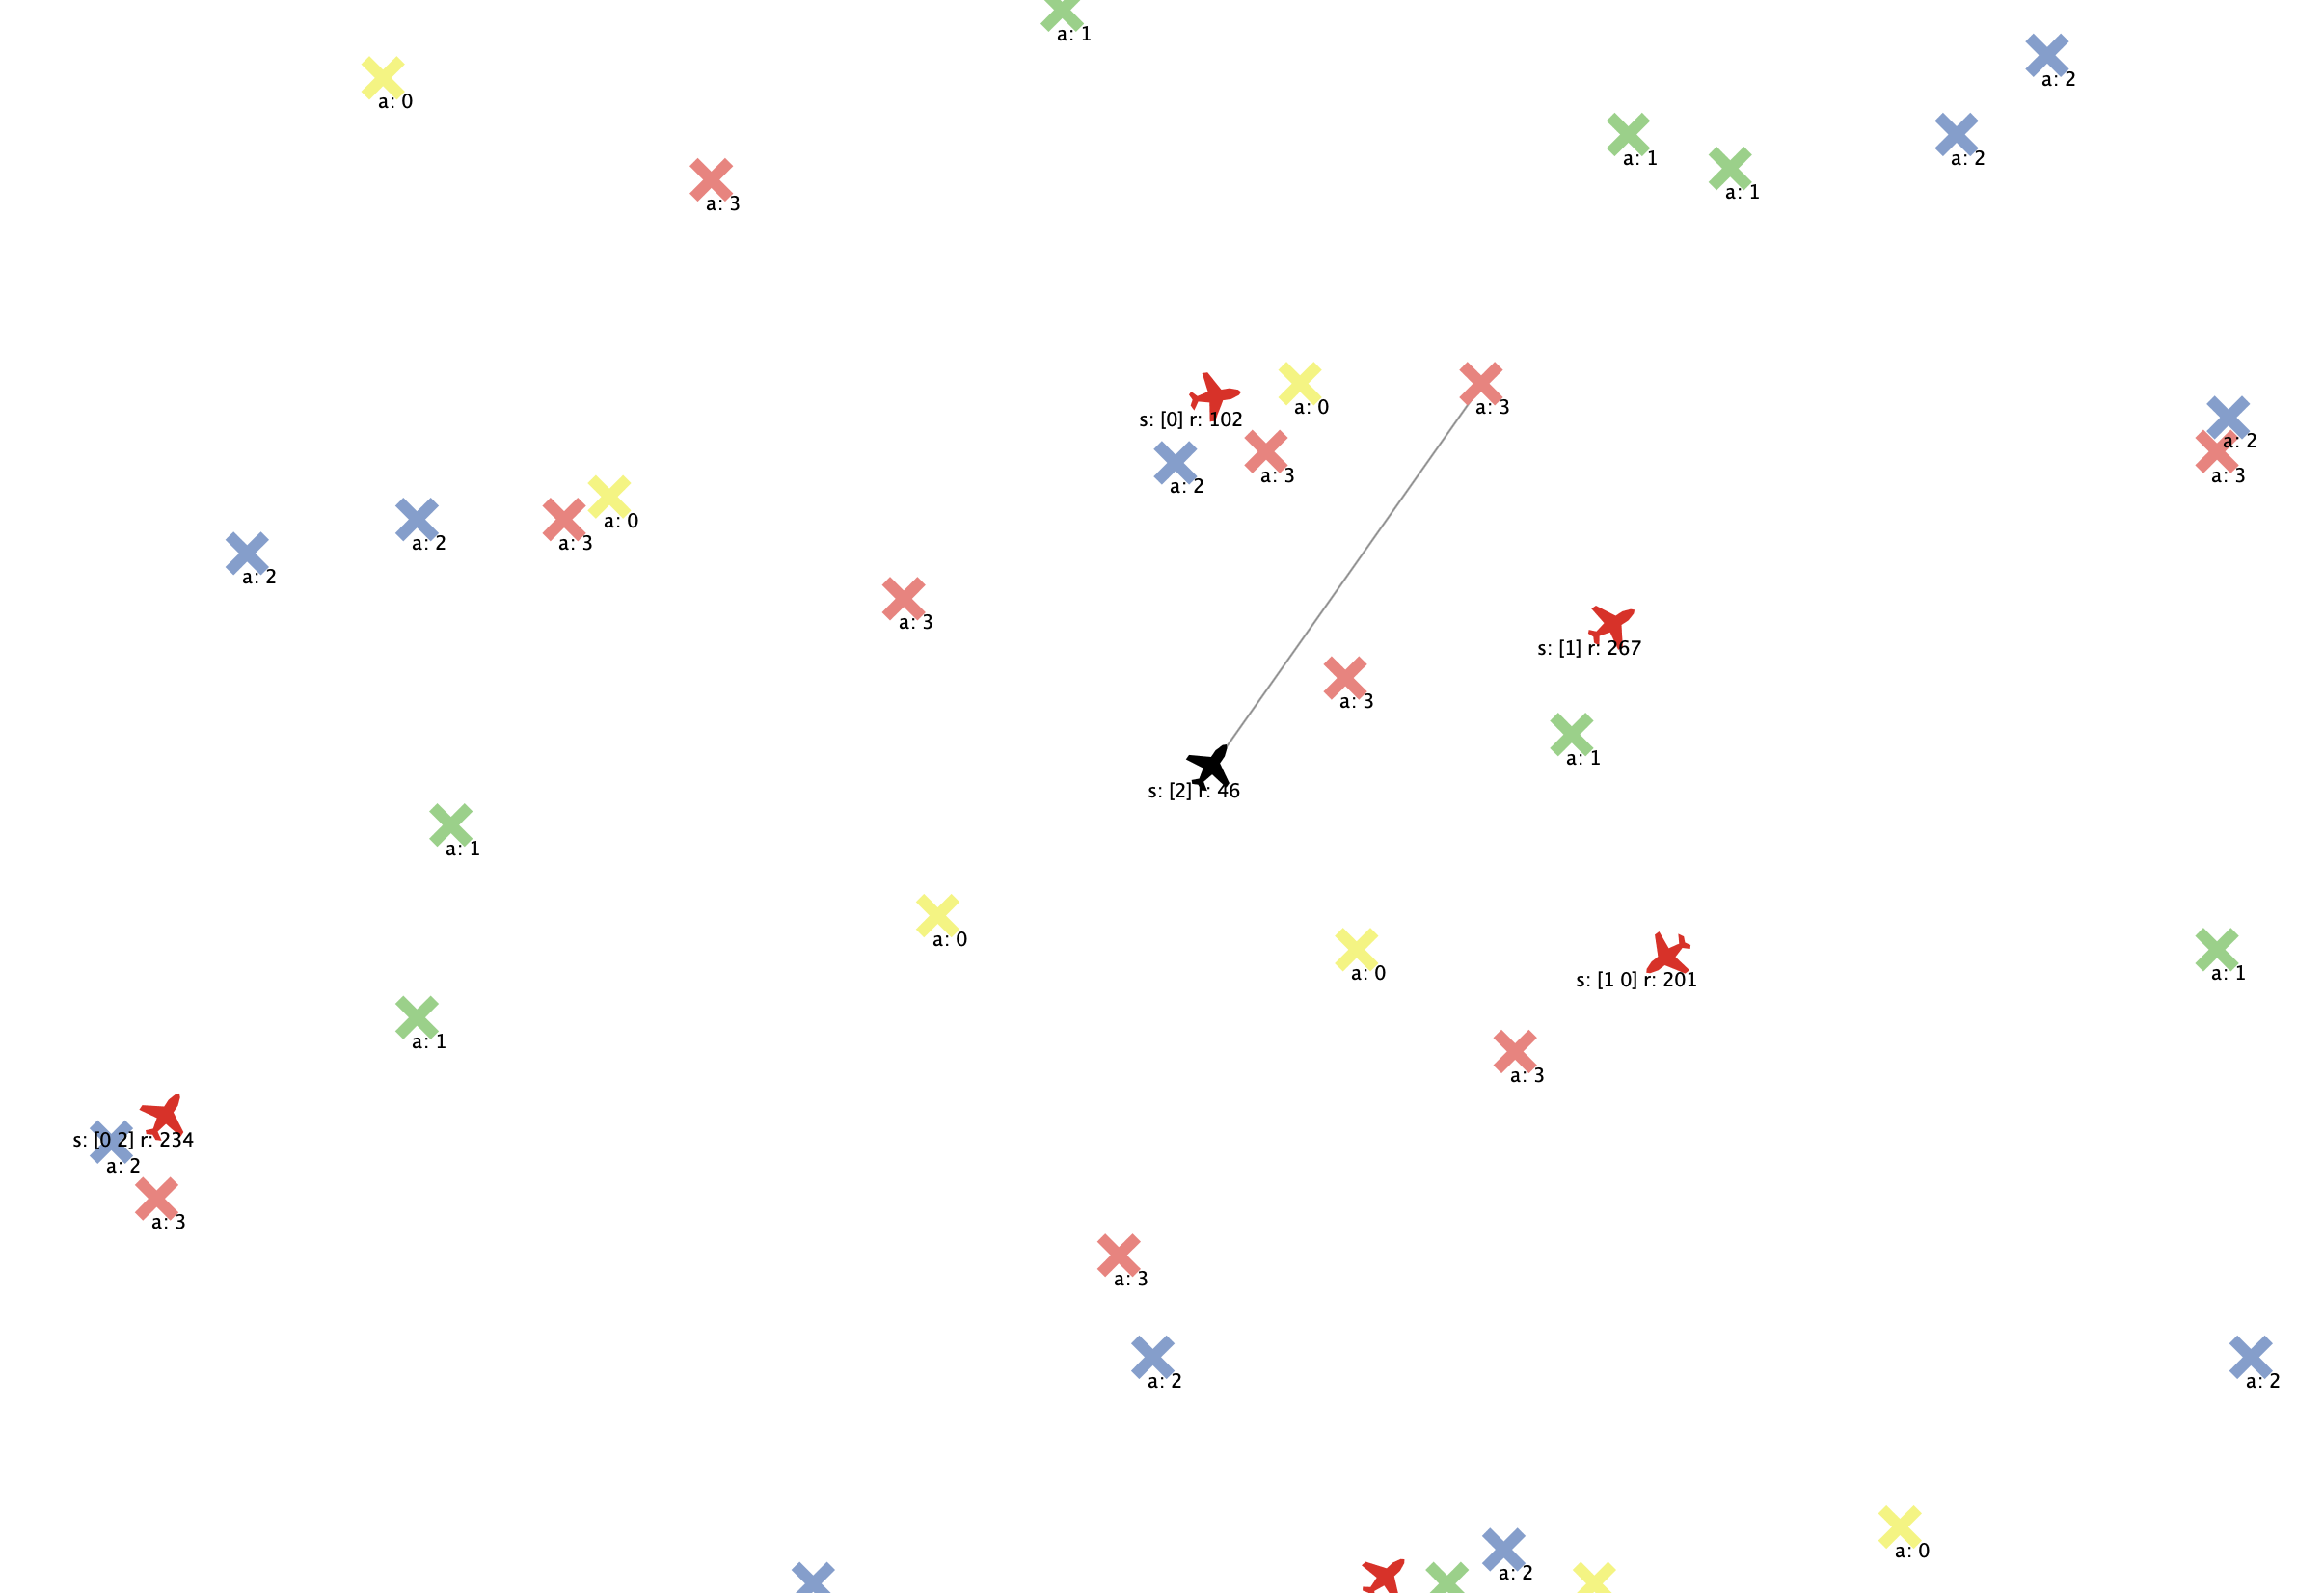
\includegraphics[scale=0.3]{fig/tela01.png}}
		\caption{NetLogo 5.3.1 screen with dropped UAVs in red, in the dynamic scenario}
		\label{fig:screen01}
	\end{center}
\end{figure}

As the number of agents changes during the execution, this new dynamic scenario supported the analysis of the agents' response and the original algorithms' assessment. However, the focus of the analysis was on the broadest scenario with 9 UAVs. It was chosen because, with small scenarios, the differences in preliminary results were not statistically significant due to high standard deviation. Furthermore, the independent replication was done with the three algorithm variants (AL, SAL and LAL) presented in Section \ref{sec:background}.

Furthermore, we updated the $stimulus$ attribute value to adjust the willingness of the agent to perform each task and analyze its impact on a dynamic context (see Line \ref{line:stimulus}). The initial value used by the original study was $0.6$ as explained in Section \ref{sec:background}, giving a good balance among distance and quality of the sensors at the choose task moment, but different values were tested to measure impacts. The results of these simulations are discussed in Section \ref{sec:discussion}. 